\section{Firmware}
Il firmware installato sul microcontroller ATmega 32U4 è stato sviluppato in C++ usando Arduino IDE, e ha i seguenti compiti:
\begin{itemize}
	\item Permettere all'applicazione di identificare i dispositivi OpenLDAT connessi e le loro capability
	\item Ricevere comandi dall'applicazione e inviare l'output via seriale
	\item Configurare l'hardware per le varie modalità di funzionamento (ADC, gain del sensore, generazione automatica o manuale dei click)
	\item Campionare il sensore (e se richiesto il bottone esterno) nel modo più veloce e regolare possibile
	\item Consentire la misurazione di metriche di velocità del dispositivo senza influire sul suo funzionamento
	\item Essere facilmente estensibile, per permettere l'aggiunta di altri sensori in versioni future del dispositivo
\end{itemize}

Il progetto si trova nella cartella \texttt{Device/Firmware/OpenLDAT} del repository, ed è composto da 4 file:
\begin{itemize}
	\item \texttt{OpenLDAT.ino}: è il file principale del firmware, importa gli altri file del progetto, implementa la ricezione dei comandi dall'applicazione e il listing delle capability
	\item \texttt{BuildConfig.h}: permette di attivare/disattivare alcune funzioni del firmware e dichiara alcune variabili globali, come il numero di versione
	\item \texttt{OscilloscopeDebug.h}: implementa delle macro che sono utilizzate all'interno del codice quando viene compilato con il debug con oscilloscopio attivo. Queste macro consentono di collegare un oscilloscopio al pin 10 della board del microcontroller e ottenere informazioni sui tempi di campionamento senza rallentare il funzionamento del dispositivo. Il funzionamento verrà discusso meglio in seguito
	\item \texttt{LightSensor.h}: contiene tutto il codice di configurazione e campionamento del sensore di luminosità, del pulsante esterno, e dei click automatici
\end{itemize}

\subsection{Formato dei comandi}
I comandi che l'applicazione può mandare al dispositivo sono composti da 2 o più byte:
\begin{itemize}
	\item Il primo byte identifica il comando. Nella versione attuale sono implementati tre comandi: \begin{itemize}
		\item \texttt{IDLE} (0x49): interrompe qualsiasi attività in corso e si prepara a ricevere un nuovo comando
		\item \texttt{ID} (0x44): invia informazioni sul dispositivo e le sue capability all'applicazione, poi si prepara a ricevere un nuovo comando
		\item \texttt{LIGHTSENSOR} (0x4C): configura il dispositivo e avvia il campionamento. L'esecuzione di questo comando continua fino a quando non viene ricevuto un nuovo comando
	\end{itemize}
	Eventuali comandi non validi vengono ignorati
	\item Il secondo byte contiene dei flag il cui significato dipende dal comando selezionato, verranno discussi in seguito
	\item Opzionalmente, possono seguire ulteriori byte di informazioni specifiche del comando selezionato. Nessuno dei comandi attualmente implementati fa uso di questa funzione
\end{itemize}

\subsection{Identificazione del dispositivo}
L'identificazione del dispositivo da parte dell'applicazione avviene in due fasi:
\begin{itemize}
	\item I dispositivi OpenLDAT vengono trovati in base all'ID hardware personalizzato. Il dispositivo si dichiara con il nome "OpenLDAT Model 1" e ID hardware (VID:PID) 4370:0001, il che lo rende facilmente distinguibile da altri dispositivi basati sulla stessa board che potrebbero essere connessi al PC. La figura \ref{fig:lsusb} mostra un output del comando \texttt{lsusb} di GNU/Linux mentre il dispositivo è connesso. Non è necessario installare nessun driver per comunicare col dispositivo
	\item Una volta stabilita la connessione, l'applicazione utilizza il comando \texttt{ID} per chiedere al dispositivo le sue capability, in base alle quale decide se il dispositivo è supportato. Il formato di questo elenco verrà discusso nel paragrafo successivo.
\end{itemize}

\begin{figure}[h]
	\centering
	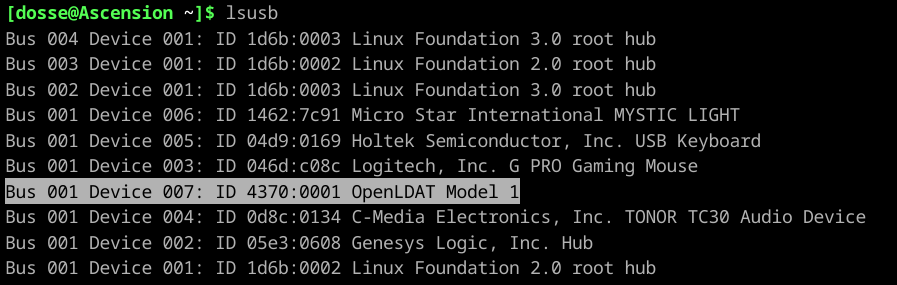
\includegraphics[width=\textwidth]{Chapter03/res/lsusb.png}
	\caption{Elenco di dispositivi USB, tra cui un OpenLDAT}
	\label{fig:lsusb}
\end{figure}

L'elenco delle capability è inviato come testo ASCII. Il seguente listato mostra un possibile output del comando \texttt{ID}.
\lstinputlisting{Chapter03/res/id_example.txt}
L'elenco è un insieme di stringhe ASCII, separate da un carattere newline (\texttt{\textbackslash n}), e terminate da una riga vuota (doppio newline). La prima riga contiene il nome completo del dispositivo, mentre le righe successive sono un elenco di capability in formato \texttt{Nome: Valore}.

Le capability attualmente implementate sono le seguenti:
\begin{itemize}
	\item \texttt{FW}: stringa contenente la versione del firmware del dispositivo, obbligatoria
	\item \texttt{LightSensor}: booleano che indica se è presente il sensore di luminosità. Se è presente, devono essere presenti anche le proprietà \texttt{LBuffer} e \texttt{SBuffer}, due interi il cui significato verrà spiegato nella sezione sul campionamento
	\item \texttt{OscilloscopeDebug}: booleano che indica se è possibile collegare un oscilloscopio al pin 10 per ottenere metriche sul timing del dispositivo
	\item \texttt{SerialDebug}: booleano che indica se il firmware è pensato per comunicare manualmente tramite il serial plotter di Arduino IDE oppure se è pensato per comunicare con l'applicazione. Rallenta notevolmente l'esecuzione del firmware
	\item \texttt{Prototype}: booleano che indica se il dispositivo è un prototipo o una versione finale. Per i prototipi sono disponibili delle funzionalità aggiuntive nell'applicazione
	\item \texttt{MinAppVer}: intero che indica la versione del driver minima richiesta da questo dispositivo, obbligatorio
	\item \texttt{SerialNo}: stringa contenente il numero di serie del dispositivo (letto dalla EEPROM), oppure \texttt{DIY} se è stato assemblato a mano
\end{itemize}

\subsection{Configurazione e campionamento del sensore}
All'accensione del dispositivo, il codice di inizializzazione avvia un'interfaccia USB HID mouse per simulare i click, e un'interfaccia seriale, così che possa comunicare con l'applicazione. Una caratteristica del microcontroller 32U4 è che utilizza l'USB CDC serial, per cui la comunicazione seriale avviene alla velocità del bus USB, e non ai baudrate della RS-232 come avviene nell'Arduino Uno. Questo consente una comunicazione molto più rapida ed evita di introdurre ritardi nel codice.

Il comando \texttt{LIGHTSENSOR} viene inviato dall'applicazione al dispositivo quando vuole utilizzare il sensore. Questo comando ha 7 possibili flag, che sono usati per configurare il dispositivo in vari modi. Considerando il byte di flag che segue il comando, partendo dal bit 0 (LSB) arrivando al bit 7 (MSB):
\begin{itemize}
	\item \textbf{Bit 0 (LSB)}: \texttt{AUTOFIRE}. Quando è impostato a 1, il dispositivo genera i click automaticamente, altrimenti li riceve dal pulsante esterno. Il valore di questo flag è ignorato se il flag \texttt{MONITOR} è impostato a 1
	\item \textbf{Bit 1}: \texttt{NOBUFFER}. Quando è impostato a 1, invia ogni sample immediatamente (più lento) anziché aspettare di aver riempito un buffer da mandare in blocco (più veloce)
	\item \textbf{Bit 2}: \texttt{HIGHSENS1}. Controlla la resistenza da 22k\si{\ohm} collegata al pin D14. Se è impostato a 1, la resistenza è attiva, aumentando il gain. Assieme al flag \texttt{HIGHSENS2} permette di selezionare 4 livelli di gain del sensore
	\item \textbf{Bit 3}: \texttt{MONITOR}. Quando è impostato a 1, viene letto il sensore ignorando i click (interni o esterni). Permette una lettura più veloce del sensore
	\item \textbf{Bit 4}: \texttt{NOCLICK}. Quando è impostato a 1, i click non vengono inviati tramite l'interfaccia USB HID mouse. I click sono comunque visibili sul LED e sull'interfaccia seriale. Il valore di questo flag è ignorato se il flag \texttt{MONITOR} è impostato a 1
	\item \textbf{Bit 5}: \texttt{FASTADC}. Quando è impostato a 1, configura l'ADC del microcontroller 32U4 per campionare molto più velocemente di quanto farebbe normalmente, consentendo velocità di campionamento fino a circa 30kHz
	\item \textbf{Bit 6}: \texttt{HIGHSENS2}. Controlla la resistenza da 47k\si{\ohm} collegata al pin D15. Se è impostato a 1, la resistenza è attiva, aumentando il gain. Assieme al flag \texttt{HIGHSENS1} permette di selezionare 4 livelli di gain del sensore
	\item \textbf{Bit 7 (MSB)}: Riservato per uso futuro (sempre 0 nella versione attuale)
\end{itemize}

Combinando i flag \texttt{NOBUFFER}, \texttt{FASTADC} e \texttt{MONITOR} in diversi modi, si possono ottenere 8 possibili velocità di campionamento, mostrate in tabella \ref{tab:openldat_samplerates}.
\begin{table}[h!]
	\centering
	\resizebox{\columnwidth}{!}{\begin{tabular}{|c|c|c|c|c|} 
		\hline
		\texttt{NOBUFFER} & \texttt{FASTADC} & \texttt{MONITOR} & \textbf{Sample rate effettivo} & \textbf{Campionamento}   \\ 
		\hline
		1 & 0 & 0 & 7796.0Hz & 100\%         \\
		\hline
		1 & 0 & 1 & 7798.0Hz & 100\%         \\
		\hline
		1 & 1 & 0 & 20710.0Hz & 100\%         \\
		\hline
		1 & 1 & 1 & 21000.0Hz & 100\%         \\ 
		\hline
		0 & 0 & 0 & 8738.1Hz (416.1buf/s) & 97.92\%         \\
		\hline
		0 & 0 & 1 & 8758.4Hz (274.4buf/s) & 98.52\%         \\
		\hline
		0 & 1 & 0 & 28896.0Hz (1376.0buf/s) & 93.12\%         \\
		\hline
		0 & 1 & 1 & 29524.4Hz (924.2buf/s) & 95.01\%         \\
		\hline
	\end{tabular}}
	\caption{\label{tab:openldat_samplerates}Velocità di campionamento}
\end{table}

Il flag \texttt{NOBUFFER} permette di attivare o disattivare il buffering sul dispositivo dei dati da mandare al PC. L'interfaccia seriale del microcontroller possiede due buffer di 64 byte (uno in ingresso e uno in uscita), e finché il buffer di scrittura non è pieno, le operazioni di scrittura su seriale non sono bloccanti, ma richiedono comunque del tempo per la copia dei dati sul buffer della seriale. Il firmware del dispositivo offre quindi una modalità con buffer, in cui il sensore viene letto il più velocemente possibile, i dati vengono messi in un buffer, e poi con una singola chiamata vengono copiati sul buffer di uscita della seriale. Questa copia avviene ogni 32 sample (\texttt{LBUFFER}) se si sta leggendo solo il sensore di luminosità, oppure ogni 21 sample (\texttt{SBUFFER}) se si sta leggendo anche il pulsante. Quando il firmware esegue la copia sul buffer della seriale, causa una breve interruzione nel campionamento, per cui la qualità del segnale catturato è leggermente inferiore in questa modalità rispetto a quella senza buffer, ma poiché vengono eseguite meno operazioni di scrittura su seriale, il sample rate effettivo è più alto.

Il formato dei dati che vengono inviati all'applicazione è diverso a seconda della configurazione scelta:
\begin{itemize}
	\item \textbf{\texttt{NOBUFFER=1}, \texttt{MONITOR=1}}: viene letto solo il sensore di luminosità, e i sample sono inviati uno per volta. Ogni sample è formato da 2 byte contenenti un intero senza segno tra 0 e 1023 (little endian)
	\item \textbf{\texttt{NOBUFFER=1}, \texttt{MONITOR=0}}: viene letto sia il sensore che il click, e i sample sono inviati uno per volta. Ogni sample è formato da 3 byte: i primi 2 byte contengono il valore del sensore di luminosità, e il terzo byte contiene 1 se in quel momento è stato premuto il pulsante, 0 altrimenti. Il segnale del pulsante è già debounced
	\item \textbf{\texttt{NOBUFFER=0}, \texttt{MONITOR=1}}: viene letto solo il sensore di luminosità, e vengono inviati all'applicazione blocchi di 32 sample di 2 byte ciascuno contenenti i valori di luminosità. In totale vengono inviati 64 byte per blocco
	\item \textbf{\texttt{NOBUFFER=0}, \texttt{MONITOR=0}}: vengono letti sia il sensore di luminosità che il click, e vengono inviati prima 21 coppie di byte contenenti i valori di luminosità, poi vengono inviati 21 byte singoli contenenti lo stato del pulsante per ogni sample di luminosità ricevuto. In totale vengono inviati 63 byte per blocco
\end{itemize}

Per massimizzare la velocità di esecuzione, queste quattro situazioni sono implementate nel firmware come quattro funzioni separate; la scelta della versione da utilizzare avviene durante il parsing del comando.

I flag \texttt{HIGHSENS1} e \texttt{HIGHSENS2} permettono di selezionare tra 4 possibili livelli di gain, mostrati in tabella \ref{tab:openldat_gains}. Il guadagno del sensore non ha effetti sulla velocità di campionamento.
\begin{table}[h!]
	\centering
	\begin{tabular}{|c|c|c|} 
		\hline
		\texttt{HIGHSENS2} & \texttt{HIGHSENS1} & \textbf{Gain}  \\ 
		\hline
		0 & 0 & 1         \\ 
		\hline
		0 & 1 & 1.258         \\ 
		\hline
		1 & 0 & 2.101         \\ 
		\hline
		1 & 1 & 13.883         \\ 
		\hline
	\end{tabular}
	\caption{\label{tab:openldat_gains}Livelli di gain implementati}
\end{table}

Quando il flag \texttt{MONITOR} è impostato a 0, il dispositivo ascolta i click in arrivo dall'esterno o generati automaticamente tramite l'utilizzo di un interrupt. Nel firmware sono presenti due ISR:\begin{itemize}
	\item Per i click automatici è sufficiente una ISR semplice che risponde all'arrivo di un segnale \texttt{HIGH} sul pin D7 e lo gestisce impostando una variabile \texttt{buttonPressed} a 1 e se necessario inviando un click tramite l'interfaccia USB HID
	\item Per i click provenienti dall'esterno è necessaria una ISR che implementi il debouncing, altrimenti per ogni pressione verrebbero registrati più click. Questa ISR più complessa si attiva all'arrivo di un segnale \texttt{HIGH} sul pin D7, esegue il debouncing di 200ms, e se passa il test imposta \texttt{buttonPressed} a 1 e se necessario simula il click
\end{itemize}

L'esecuzione delle ISR non rallenta significativamente il campionamento, in quanto richiedono pochi microsecondi per essere eseguite.\\
Per massimizzare la velocità di esecuzione, queste due ISR sono in realtà implementate nel firmware come quattro ISR: due semplici (con e senza simulazione del click), e due con debouncing (con e senza simulazione del click). La scelta dell'ISR da usare avviene durante il parsing del comando.

L'invio dei click del mouse avviene tramite la libreria HID-Project di NicoHood\footnote{\href{https://www.arduino.cc/reference/en/libraries/hid-project/}{https://www.arduino.cc/reference/en/libraries/hid-project/}}, scaricabile tramite il gestore di librerie di Arduino IDE.

Attenzione: l'arrivo di un interrupt causa inevitabilmente un'interruzione del campionamento, ma poiché la durata delle ISR è così breve, ed è un ordine di grandezza più piccola dei valori che vogliamo misurare, l'applicazione può ignorare questi "buchi" nel campionamento senza perdere precisione.

La generazione automatica dei click, se richiesta con il flag \texttt{AUTOFIRE}, avviene configurando il timer 4 del microcontroller 32U4 per generare un segnale a circa 1Hz che esce dal pin D6 e entra direttamente nel pin D7, lo stesso da cui entrano i click esterni e collegato al LED frontale. La configurazione di questo timer non influisce su nessun'altra funzione di Arduino utilizzata nel firmware. Utilizzando questo sistema, inoltre, non si rallenta il firmware (ad eccezione dell'occasionale interrupt).\\
Il timer 4 è un timer a 10 bit configurabile tramite un set di registri\cite{atmega32u4_datasheet}, e viene configurato in questo modo: output sul pin D6, ciclo completo dei 1024 valori del contatore, segnale \texttt{HIGH} quando il contatore è sotto il valore di 64, prescaler impostato al valore massimo di 16384, conteggio che parte da 0. Il risultato è un'onda quadra con un periodo di circa 1.048576s e un duty cycle del 6.25\%, perfetta per generare interrupt periodici.\\
Durante la configurazione vengono disattivati gli interrupt per evitare di generare click accidentali.

Il flag \texttt{FASTADC}, se impostato a 1, permette di campionare il sensore di luminosità molto più velocemente del normale, seppur con alcune limitazioni. L'ADC del microcontroller 32U4 è composto da due parti: un ADC ad approssimazioni successive (SAR) e un circuito sample and hold che carica un condensatore da 14pF che mantiene il valore da campionare mentre l'ADC esegue il suo compito.\\
Normalmente, l'esecuzione di una \texttt{analogRead} richiede circa 112us, il che limita la frequenza di campionamento a circa 8.9kHz, e una volta considerato il processamento che va fatto per memorizzare e inviare il sample, la frequenza di campionamento è limitata a circa 7kHz. Leggendo la documentazione del microcontroller 32U4, si scopre che alterando il registro \texttt{ADCSRA} è possibile variare il clock dell'ADC dal default di 125kHz fino un massimo di 1MHz\cite{atmega32u4_datasheet}, a costo di due limitazioni: una maggiore sensibilità a rumori di conversione, e un'impedenza massima del segnale da campionare drasticamente ridotta poiché il condensatore del circuito sample and hold ha meno tempo di caricarsi.\\
Nel firmware del dispositivo, quando il flag \texttt{FASTADC} è impostato a 1, il clock viene portato a 500kHz, ottenendo così un tempo di circa 30us per \texttt{analogRead} (dai 112us originali), per una frequenza massima teorica di campionamento di circa 33.2kHz, che scende a circa 30kHz una volta aggiunto il tempo di processamento. L'impedenza del sensore è abbastanza bassa da non creare problemi a questa velocità di campionamento, indipendentemente dal livello di gain selezionato. La rumorosità del segnale catturato non sembra essere alterata in questa modalità nella versione finale del dispositivo assembato su PCB, ma era misurabile a circa 1-2 bit nei primi prototipi assemblati su schede millefori, poiché captavano molte più interferenze dall'esterno.

\subsection{Debugging e misurazione delle tempistiche}
Per permettere un debugging più semplice del firmware utilizzando solo Arduino IDE, è stato aggiunto il flag di compilazione \texttt{SERIAL\_DEBUG}. Quando questo flag è abilitato, il firmware non genera output nel formato binario per l'applicazione, ma in formato testuale, compatibile con il serial monitor e il serial plotter di Arduino IDE. Questo rallenta notevolmente il campionamento, per cui qualsiasi misurazione fatta in questa modalità è da considerarsi invalida, e l'applicazione rifiuta il collegamento se questa modalità è attiva.\\
In questa modalità, inoltre, il firmware accetta comandi sia nel formato binario dell'applicazione che in testo esadecimale (solo comandi da 2 byte). Per inviare un comando esadecimale, basta anteporre un carattere \texttt{x} minuscolo all'inizio del comando, ad esempio il comando \texttt{x4400} chiede al dispositivo di identificarsi (\texttt{44} è il comando \texttt{ID}, \texttt{00} è un byte di flag vuoto), e il comando \texttt{x4C2E} avvia il campionamento con i flag \texttt{MONITOR}, \texttt{FASTADC} e \texttt{NOBUFFER} impostati ad 1 e livello di gain medio.\\
La figura \ref{fig:serialdebug} mostra un esempio di output sul serial plotter.

\begin{figure}[h]
	\centering
	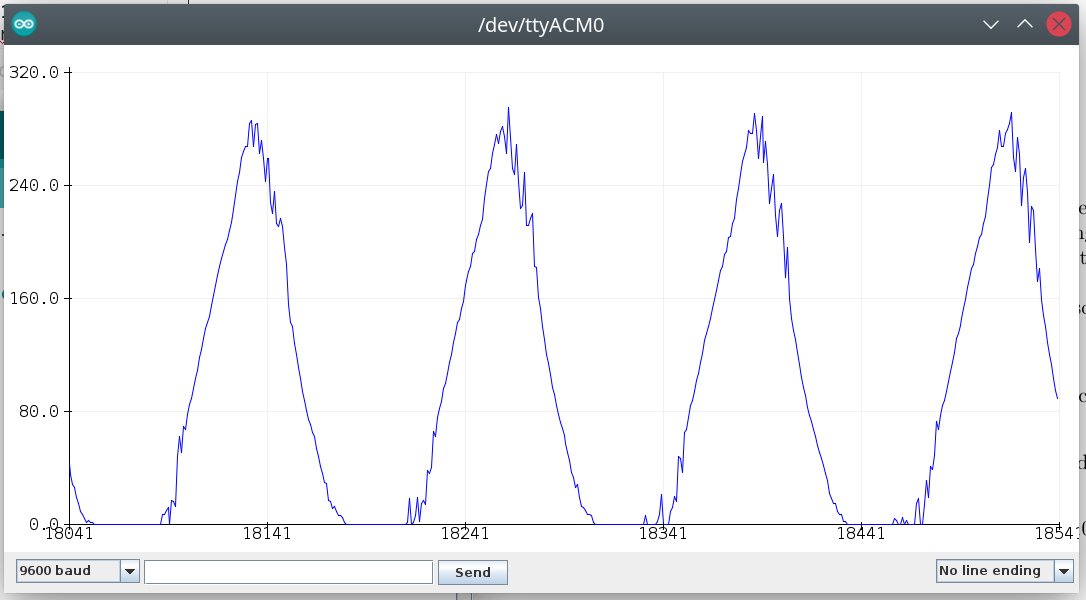
\includegraphics[width=\textwidth]{Chapter03/res/serialdebug.png}
	\caption{Esempio di output su serial monitor. (Nota: in questo esempio il sensore non era collegato, quindi il grafico mostra interferenze provenienti dall'esterno)}
	\label{fig:serialdebug}
\end{figure}

Per misurare le tempistiche di esecuzione del firmware (e in particolar modo, determinare il sample rate nelle varie modalità) non si può semplicemente fare una differenza tra timestamp e stamparla su seriale, poiché questo rallenterebbe troppo l'esecuzione, per cui la tecnica che viene implementata quando il firmware è compilato col flag \texttt{OSCILLOSCOPE\_DEBUG} è quella di generare un segnale che è \texttt{HIGH} mentre il firmware sta leggendo il sensore, e \texttt{LOW} mentre sta scrivendo sulla seriale (o viceversa); collegando un oscilloscopio all'uscita di questo segnale è possibile misurarne la frequenza (e quindi il sample rate) e verificare anche la presenza di "buchi" nel campionamento. Con la stessa tecnica è possibile misurare i tempi di esecuzione delle ISR.\\
La generazione di questo segnale non può essere fatta utilizzando funzioni come \texttt{digitalWrite} poiché richiedono parecchi microsecondi per essere eseguite e questo invaliderebbe completamente la misura. Studiando la documentazione del microcontroller 32U4 si scopre la presenza di una funzione speciale del pin 10: quando il bit 6 del registro \texttt{PINB} viene scritto ad 1, il valore corrente di quel pin viene invertito\cite{atmega32u4_datasheet}. Scrivere il registro \texttt{PINB} richiede un singolo ciclo di clock, che corrisponde a 62ns, un ordine di grandezza inferiore ai tempi che stiamo cercando di misurare.\\
Per rendere facilmente utilizzabile questa funzione nel firmware, sono state realizzate tre macro:
\begin{itemize}
	\item \texttt{OSCILLOSCOPE\_DEBUG\_INIT()}: inizializza il pin 10 come output e con un segnale \texttt{LOW}
	\item \texttt{OSCILLOSCOPE\_DEBUG\_PULSE()}: inverte il valore del pin 10 manipolando il registro \texttt{PINB}
	\item \texttt{OSCILLOSCOPE\_DEBUG\_END()}: reimposta in pin 10 ad alta impedenza e cancella lo stato \texttt{HIGH} o \texttt{LOW}
\end{itemize}
Nella versione finale del firmware, queste macro sono usate per generare una pulsazione per ogni sample (con flag \texttt{NOBUFFER} impostato a 1) o per ogni buffer (senza flag \texttt{NOBUFFER}). In modalità con buffering, per ottenere il sample rate, la frequenza del segnale generato va moltiplicata per la dimensione del buffer (32 se il flag \texttt{MONITOR} è impostato a 1, altrimenti 21).

La figura \ref{fig:oscilloscopedebug} mostra un esempio del segnale generato da questa modalità di debugging. Il dispositivo stava operando con \texttt{NOBUFFER=1}, \texttt{MONITOR=1}, \texttt{FASTADC=1}, per un sample rate di 21000Hz. Piccole variazioni della frequenza di questo segnale sono perfettamente normali, e possono avvenire in seguito a interrupt (click automatici o esterni) o semplicemente per variazioni sul segnale di clock; non influiscono in maniera rilevante sulle misurazioni fatte dall'applicazione.

\begin{figure}[h]
	\centering
	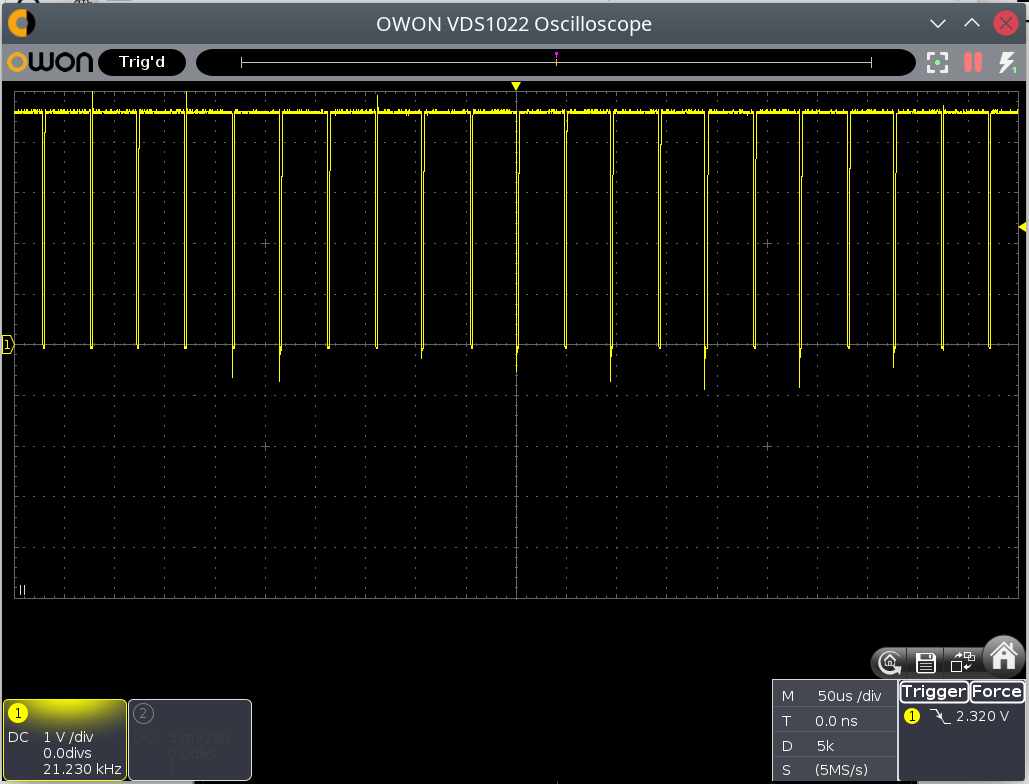
\includegraphics[width=\textwidth]{Chapter03/res/scope.png}
	\caption{Esempio di segnale generato da \texttt{OSCILLOSCOPE\_DEBUG}}
	\label{fig:oscilloscopedebug}
\end{figure}

Attenzione: le velocità di campionamento possono variare leggermente a causa degli aggiornamenti del compilatore GCC e delle librerie Arduino. Per questo motivo viene fornito un firmware precompilato in formato .hex flashabile con il tool avrdude.
